%!TEX root = main.tex
\documentclass[main.tex]{subfiles}

\begin{document}


\chapter{Introduction}

\setlength{\epigraphwidth}{0.75\textwidth}
\renewcommand{\textflush}{flushepinormal}
\epigraph{The major challenge for language documentation in the next decade or two is what could be called the transcription challenge. This is a multilayered challenge that goes far beyond the practical challenge of speeding up the transcription process. [...] Despite its centrality to language documentation, transcription remains critically undertheorized and understudied. Further progress in language documentation, and ultimately also its overall success, crucially depends on further investigating and understanding the transcription process, broadly conceived.}%
         {\justifying\fullcite{himmelmann2018meeting}}

Language documentation is typically considered a sub-field of linguistics and its goal is ``to provide a comprehensive record of the linguistic practices characteristic of a given speech community'' \parencite[][p.~166]{himmelmann1998documentary}.~Many aspects of its practice, however, require continual integration of developments beyond linguistics.~As the target languages are often spoken by minoritised Indigenous communities, it is necessary to proactively consider evolving norms regarding fair and ethical collaboration \parencite{holton2022indigenous}.~Concurrently, data protocols must not only continually integrate these norms but also technological advancements that more effectively enable the creation, processing, storage, and distribution of recorded materials \parencite{berez2023recent}.~In both respective areas, there are ongoing developments that constitute paradigm shifts:~1) decolonising, community-centred approaches to working with Indigenous communities, and 2) speech and language processing systems powered by foundation models (FMs).~Integrating considerations from the former and leveraging advancements in the latter, I examine in this dissertation how these FM-powered systems can help create contextually-appropriate solutions to combat a major bottleneck in language documentation workflows --- the transcription of recorded materials.

\section{Language documentation and the transcription bottleneck}

It is generally recognised that there are about 7,000 languages spoken in the world today and that at least half of them may not exist by the end of the century \parencite{austin2011cambridge}.~Many of these languages are spoken by Indigenous and minoritised communities, who are under cultural, economic, and technological pressures to shift to using more dominant regional, national, or global languages.~For example, education may be conducted entirely in more widely-used regional or national languages and technological interfaces may only exist in a national or global language.~Such pressures can lead to language endangerment, as younger generations gradually adopt the more widely-used languages until there remain no living first-language or `L1' speakers, at which point a language may become `dormant'.

There are many ongoing revitalisation efforts to fight these pressures by encouraging the learning and active use of endangered languages, safeguard the knowledge of elder L1 speakers by recording them, as well as efforts to ‘awaken’ dormant ones based on archival recordings.~However, as recording speech is considerably easier than transcribing the recorded speech, many recording collections of these languages remain only partially transcribed, if at all \parencite{cox2019taking}.~Yet, raw audio data comprising untranscribed speech is difficult to index and search, limiting how efficiently content within the materials can be discovered and used (e.g.~for creating language learning materials).~Indeed, the difficulty is so ubiquitous that it has been termed the ``transcription bottleneck'' \parencite[]{seifart2018language,foley2018building,cox2019taking}, and the consequences of hard-to-access materials so dire that there are warnings against inadvertently creating ``data graveyards, i.e. large heaps of data with little or no use to anyone'' \parencite[][p. 4]{himmelmann2006language}.

There are several contributing factors that result in this bottleneck with respect to transcribing minoritised languages.~First, unlike major languages such as English, searchable high-quality transcriptions cannot simply be derived using a high-performance automatic speech recognition (ASR) system, whose development itself has conventionally required large quantities of transcribed speech.~Second, there is typically no option for large-scale crowd-sourcing of target language transcriptions as by definition of endangerment there may be very few speakers and only a subset of speakers may be literate in this language (i.e.~not the regional or national language of formal education).~Third, there may not be a standardised orthography for the target language, in which case a project-specific working orthography is often developed, resulting in transcriptions with both intra- and inter-transcriber variation, requiring additional time for review and corrections.~Finally, in some instances, there may also be an additional personnel bottleneck resulting from limitations on who can listen to and transcribe certain recordings (e.g.~of culturally-sensitive materials such as descriptions of ceremonial procedures).~Taken altogether, surveys of transcription time have reported typically requiring about 30 to 50 hours of work to transcribe one hour of recorded speech \parencite{durantin2017survey,michaud2014towards,zahrer2020towards}.

Language documentation and description are considered two inter-dependent but different activities varying in outputs and goals \parencite{himmelmann1998documentary}.~Language documentation, which includes data collection, transcription and translation, aims to produce a multi-purpose record of a language.~Its outputs are primary data that may be useful to a broad audience, including community members, language teachers, anthropologists, and those from other disciplines.~The outputs of language description are typically grammatical descriptions and theoretical analyses based on these descriptions that are more narrowly aimed at comparative linguists.~Historically, documentation processes have privileged the latter, which can result in primary data that is sub-optimal or inapplicable for other uses.~For example, description-focused data collection may lead to the collection of idealised forms of phenomena-of-interest rather than colloquial or child-directed speech \parencite{rouvier2017language}, the latter two of which are more relevant to revitalisation efforts.~Spurred on in part by broader decolonial efforts by Indigenous communities, community-based and collaborative documentation methods that also contribute to community needs are emerging as best practices in linguistic research \parencite{holton2022indigenous}.

\begin{figure*}[b]
  \centering
  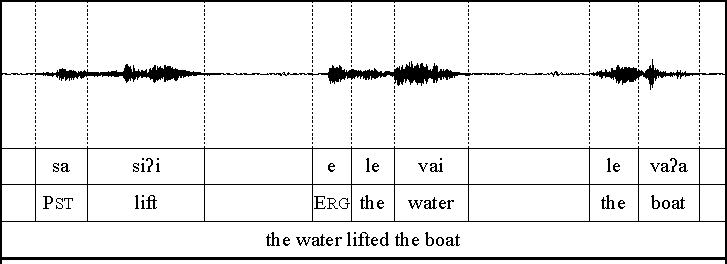
\includegraphics[width=0.7\linewidth]{figures/intro-conventional-transcription}
  \caption{A contiguous transcription of a Samoan utterance for linguistic analysis.}
\label{fig:how-lift-boat-tf}
% \vspace{-1em}
\end{figure*}

Reviewing a century of transcription practice within linguistics, \textcite{bird-2020-sparse} argues that several parts of the transcription bottleneck result from a description- and analysis-centred transcription practice, which he terms `contiguous' and suggests supplementing it with a more `sparse' approach to facilitate search and retrieval.~He identifies three inefficient characteristics particular to orthodox transcription practice:~1) transcribing phones,~2) transcribing fully, and 3) transcribing first (and translating second).~We review these characteristics using a Samoan utterance sourced from my Field Methods class recordings, illustrated in Figure \ref{fig:how-lift-boat-tf}.~Given my goal of grammatically analysing a language largely unknown to me, I am primarily interested in textually representing the form of the spoken utterance, leading to a primary focus on the phonetic form of the whole utterance [{\fontspec{LinLibertine.ttf}sasiʔielevailevaʔa}], with the translation secondary.~Using these annotations along with other data points, I can hypothesise what the various lexical and grammatical units are in Samoan and how they interact,~e.g. [{\fontspec{LinLibertine.ttf}sa}]+[{\fontspec{LinLibertine.ttf}siʔi}] P{\footnotesize{}ST}+lift `lifted'.

\begin{figure*}[t]
% \vspace{-1em}
  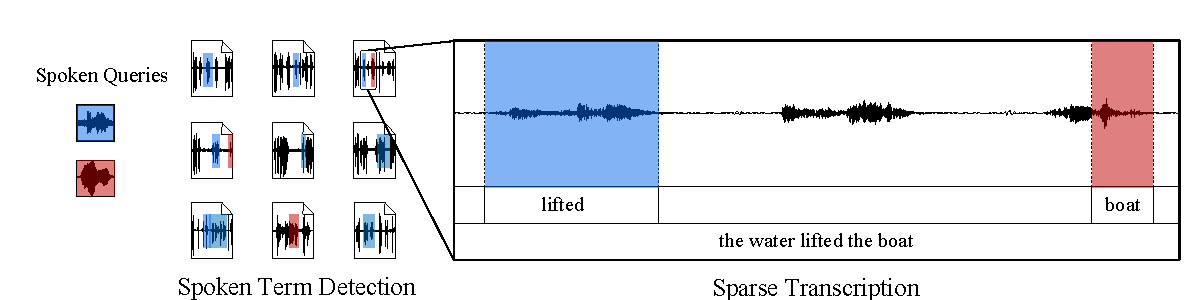
\includegraphics[width=1.0\linewidth]{figures/intro-sparse-transcription}
  \caption{A sparse transcription of a Samoan utterance for iterative and collaborative indexing.}
  \label{fig:how-lift-boat-sparse}
\end{figure*}

\begin{figure*}[b]
  \centering
  % \vspace{1em}
  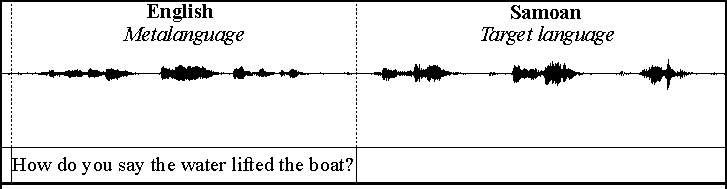
\includegraphics[width=0.7\linewidth]{figures/intro-mixed-corpus.pdf}
  \caption{Sparse transcription via automatic isolation and machine transcription of a more widely used metalanguage in a mixed-language corpus.}
  \label{fig:mixed}
\end{figure*}

\textcite{bird-2020-sparse} questions whether this conceptualisation of transcription effectively serves the many parties interested in working with untranscribed language documentation corpora, particularly those of unwritten, oral languages.~Intended as a supplementary approach, \textcite{bird-2020-sparse} proposes `sparse transcription' which does away with the three characteristics that contribute to the bottleneck in contiguous transcription and, importantly, facilitates access to untranscribed language documentation corpora in ways that are more compatible with the skills of the speech communities.~As illustrated in Figure \ref{fig:how-lift-boat-sparse}, spoken term detection or `word spotting' is used to facilitate searches via spoken queries (i.e.~a voice-based alternative to text queries on transcriptions) and, upon confirmation of hits, translations can be provided in the language of wider communication (i.e.~one in which speakers are literate).~In this way, bottlenecks relating to the need for text transcriptions, a target language orthography and literacy in target language can be removed.~The confirmed locations of various queries along with their translations allow for the corpus to be collaboratively and iteratively indexed, albeit sparsely.~Additionally, this approach can help more effectively find regions of interest to which more time-consuming contiguous transcription efforts can be strategically directed. 

Following the proposal of the sparse transcription model by \textcite{bird-2020-sparse}, there have been several studies investigating its potential in various workflow configurations and documentation scenarios (Lane \& Bird, \citeyear{lane2021local,lane2022finite}; Le Ferrand et al., \citeyear{leferrandEnablingInteractiveTranscription2020,le2021phone,le2022learning}).~One area that has been identified for improvement is the robustness of the spoken term detection system, particularly for scenarios where the speaker of the query is different to the speakers in the corpus and when the audio of the corpus is relatively noisy.~We return to this discussion below in our review of foundational models for speech and subsequent investigation of whether these models help deliver more speaker-invariant and noise-robust spoken term detection systems.

Even without a robust spoken term detection system, it may nevertheless be possible to derive a searchable index for mixed-language documentation corpora where the target language being documented is inter-mixed with a more widely spoken language for metalinguistic questions and commentary.~As illustrated in Figure \ref{fig:mixed}, the target language response by the Samoan speaker was preceded by my elicitation prompt in English:~\textit{How do you say ``the water lifted the boat''?}~As mentioned above, it is relatively straightforward to derive searchable high-quality transcriptions using a high-performance ASR system for major languages such as English.~As such, if foundation models can be used to automatically isolate and transcribe the more widely used language, these searchable metalanguage transcriptions could provide approximate locations where certain target language words and topics are being discussed this genre of mixed-language corpora which are common in language documentation.

Ultimately sparse transcription is intended as a way to ``accelerate [the work of] orthodox, contiguous transcription'' \parencite[p.~737]{bird-2020-sparse} while also facilitating immediate access to untranscribed speech corpora.~If, on one hand, sparse transcription can help efficiently gather the target language transcriptions and, on the other, foundation models can be used to substantially reduce the amount of target language transcriptions required to begin ASR system development, this combination could provide a pathway for creating ASR-assisted transcription workflows for minoritised languages.

\section{Foundation models for speech processing}

Foundation models (FMs) are a general class of models for building artificial intelligence (AI) systems.~Across many applications, they have led to a paradigm shift in AI system development \parencite{bommasani2021opportunities}.~In contrast to training a model completely from scratch, an already trained (or `pre-trained') foundation model is used as a starting point, from which this model is further trained (or `fine-tuned') for a specific task.~One major benefit of this paradigm is that pre-trained FMs enable system development with substantially smaller quantities of task-specific data (e.g.~transcriptions for ASR system development).~For example, in their proposal of wav2vec 2.0 (a framework for building foundation models for speech processing), \textcite{NEURIPS2020_92d1e1eb} demonstrated that using one hour of transcribed English to fine-tune a pre-trained wav2vec 2.0 model for ASR outperformed the previous state-of-the-art trained from scratch using 100 hours of transcribed English speech.~They further demonstrated that as little as 10 minutes of transcribed speech may suffice to begin ASR development if supplemental text data is available (e.g.~to train a language model).

~A common characteristic of FMs is that they are pre-trained in at scale in a self-supervised manner \parencite{bommasani2021opportunities}, which helps reduce the need for task-specific data in the subsequent, supervised fine-tuning stage.~In machine learning terminology, \emph{supervision} refers to human-generated labels (e.g.~human transcriptions for audio recordings), which are expensive and time-consuming to collect.~In self-supervised pre-training, the model is first trained on a proxy task (for which it can derive its own labels), after which the resulting model can be fine-tuned for the target task using human-generated labels.~Not constrained by the need to collect human labels, self-supervision enables for models to be trained at substantially larger scales than before.~Since the release of the original English wav2vec 2.0 model pre-trained on 960 hours of English audio \parencite{NEURIPS2020_92d1e1eb}, there have also been massively multilingual variants leveraging tens or hundreds of thousands of hours of audio from many languages:~XLSR-53, pre-trained on 56k hours from 53 languages \parencite{conneau2020unsupervised}; XLSR-128, pre-trained on 436k hours from 128 languages \parencite{babu2021xls}; and MMS, pre-trained on 491k hours from 1,406 languages \parencite{pratap2023scaling}.

\begin{figure*}[t]
% \vspace{-1em}
\centering
  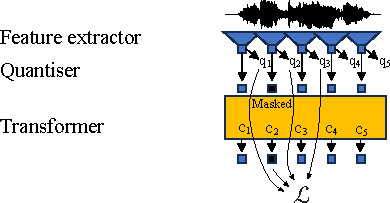
\includegraphics[width=0.45\linewidth]{figures/w2v2-intro}
  \caption[Illustration of the wav2vec 2.0 architecture.]{Illustration of the wav2vec 2.0 architecture. Adapted from \textcite{NEURIPS2020_92d1e1eb}.}
  \label{fig:intro-w2v2}
\end{figure*}

We introduce here a high-level summary of the wav2vec 2.0 framework (with additional details introduced as necessary in the chapters below).~As illustrated in Figure \ref{fig:intro-w2v2}, the wav2vec 2.0 framework leverages the transformer model architecture \parencite{vaswani2017attention}, which excels at learning how various discrete units in a sequence co-occur (e.g.~words in a sentence).~The feature extractor and quantiser are used to summarise and discretise the information in the continuous audio signal input, after which the transformer is used to learn more contextualised representations ($c_1, ..., c_5$).~To encourage the learning of such representations, the model is partly optimised using a masked modelling objective where it must correctly predict information about masked positions based on the neighbouring (unmasked) context.~Such objectives are found in many FM pre-training tasks and are akin to a Cloze test: ``\emph{I got drenched in the \_\_\_\_\_ because I forgot to take my \_\_\_\_\_}''.~Crucially, by simply masking spans within the input data, the training process can automatically derive correct task labels (e.g.~Position 1: \emph{rain},~Position 2: \emph{umbrella}).~By eliminating the need for human labelling, these models can be trained at extremely large scales (e.g.~using 436k hours of untranscribed speech for wav2vec 2.0 XLSR-128).

The representations learned by the wav2vec 2.0 transformer network have been found to be particularly useful for speech applications requiring fine-grained comparisons of acoustic-phonetic content, e.g.~second language (L2) pronunciation scoring \parencite{bartelds2022neural,richter2023relative} or spoken dialect classification \parencite{bartelds2022quantifying,guillaume23_sigul}.~For example, \textcite{bartelds2022neural} found that representations extracted from a middle layer of the transformer network were particularly robust to inter-speaker and -recording differences in the audio data being compared (i.e.~a sample recording of an L2 speaker vs.~a reference recording of the same utterance by an L1 speaker), allowing for automatic derivation of L2 pronunciation scores that closely matched the costly-to-derive human expert ratings.~Given these characteristics, a natural question that arises is whether these representations may also prove useful for improving spoken term detection performance and better enable search and retrieval of content in untranscribed language documentation corpora.

Similar information retrieval objectives may be achievable even without spoken term detection for mixed-language corpora containing both a target language and a more widely-used language such as English.~For example, utterances in the more widely-used language could be isolated by using a few utterances of each language to adapt a pre-trained spoken language identification model \parencite[e.g.~SpeechBrain:][]{ravanelli2021speechbrain}.~Utterances identified as being in the more widely-used language can then be transcribed using a high-performance ASR model for that language \parencite[e.g.~wav2vec 2.0 Robust for English:][]{hsu2021robust}.~These relatively high-quality machine-derived transcripts could then be used for plain text searches to obtain approximate time regions in which various target language words and topics are being discussed.~Thus, a natural question that arises is whether few-shot adaptation of these models can be used to help index mixed-language corpora of this genre.

As mentioned, sparse transcription is intended to supplement orthodox, continuous transcription in a way that not only accelerates the latter but also simultaneously helps to improve immediate access to documentation corpora.~In other words, once some transcriptions have been gathered, there remains questions of how to leverage foundation models to most effectively use those gathered transcriptions to begin ASR development.~In particular, we examine two questions of particular interest, both of which relate to how other available resources could also be leveraged to further increase the overall effectiveness. 

The first question relates to the use of target language text data.~As mentioned, \parencite{NEURIPS2020_92d1e1eb} demonstrated that ASR system development may be possible with as little as 10 minutes of transcribed speech if an external text corpus could be used to derive a lexicon that helps restrict the ASR system output to possible words (e.g. \emph{dogs} vs. \emph{*dogz}) as well as an \emph{n}-gram language model that also biases outputs to more probable word sequences (e.g.~\textit{two dogs} vs. \textit{too dogs}).~Given that many languages are digitally under-represented, there may only be scant amounts of text data compared to that available for English \parencite[e.g.~an 803 million word corpus as used in][]{NEURIPS2020_92d1e1eb}.~Further, for some oral languages, the documentation project's own transcriptions or elicitation wordlists in the project-developed orthography may comprise the entirety of all existing written materials in the language.~In other words, a question that remains unanswered is what the minimum amount of supplemental text data is in order to begin ASR system development when only 10 minutes of transcribed speech is available.

The second question relates to the use of untranscribed speech --- both in the target language and in similar ones.~Unlike for major languages such as English for which several monolingual wav2vec 2.0 models exist, one of the massively multi-lingual variants is typically the appropriate option for use as the foundation model for ASR fine-tuning.~However, as European languages are over-represented in the pre-training data of such models (416k of 436k = 95\% in the case of XLSR-128), fine-tuning these models for ASR for under-represented languages results in relatively lower performance compared to their over-represented counterparts \parencite{conneau2023fleurs}.~While recent studies have shown that continued pre-training (CPT) using untranscribed speech from the target language can help ameliorate this performance gap \parencite[e.g.~][]{NOWAKOWSKI2023103148,paraskevopoulos2024sample}, they involved using 70–200 hours of target language data.~For some languages, it may be quite difficult to source this much speech data --- even untranscribed.~In other words, a question that remains unanswered is whether similarly successfully CPT-based adaptation could be successfully achieved by supplementing limited amounts of target language data with data from a similar, higher-resource one (henceforth a `donor' language).

This second question, however, raises another one --- how do we determine what is a `similar' donor language is for the goal of successful CPT-based adaptation?~Recall that wav2vec 2.0 is a transformer-based model, which is designed to excel at learning how discrete units co-occur and that the pre-training objective requires learning about those co-occurrences.~In other words, it may be that the relevant linguistic properties for determining similarity are related to phonological inventory (i.e.~meaningful speech units in a language) and phonotactics (i.e.~the permissible ways in which those units can be combined).~For many under-described languages, however, there may not already be a phonological analysis that describes these properties and, further, it is impractical to manually conduct pairwise comparative analyses between a target language and its candidate donors --- warranting a bottom-up acoustic similarity measure.~Recall that the pre-trained wav2vec 2.0 model's representations are useful for fine-grained comparisons of speech, including spoken dialect classification \parencite{bartelds2022quantifying,guillaume23_sigul}.~In other words, a natural question that arises is whether these representations could be used to successfully rank the candidate donors where success is defined by the correlation of this ranking to improvements in target language ASR performance after CPT-based adaptation using a mix of data from both languages.

\begin{table}[!b]
\centering
\renewcommand{\arraystretch}{1.35}
\scalebox{0.95}{\begin{tabular}{ccll}
\toprule
\makecell[c]{\textbf{Chapter}\\{ }} & \makecell[c]{\textbf{Transcriptions}\\{\footnotesize(target lang.)}} & \makecell[l]{\textbf{Corpus type}\\{}}                                 &  \makecell[l]{\textbf{Other resources}\\{}} \\ \hline
\multicolumn{4}{l}{\hspace{0.5em}Goal: \emph{Indexing of untranscribed corpora}}\\
2 & -              & Monolingual (target language)          & -                         \\ 
3 & -              & Mixed (target language + metalanguage) & SLI model \& Metalanguage ASR \\
\multicolumn{4}{l}{\hspace{0.5em}Goal: \emph{Effective use of target language transcriptions for ASR development}}\\
4 & 10 min.        & Monolingual (target language)          & Target language texts           \\
5 & 1 hr            & Monolingual (target language)          & Donor language speech           \\
\bottomrule
\end{tabular}}
\caption{Language documentation scenarios according to amount of available transcriptions and composition of speech corpus addressed in the different chapters in the dissertation.~Initialisms: Spoken Language Identification (SLI), Automatic Speech Recognition (ASR).}
\label{tab:chapters}
\end{table}

I address all the questions posed above in the remaining chapters, summarised in \ref{tab:chapters}.~These chapters may be divided into two groups: those examining how to enable indexing without target language transcriptions (2--3) and the others examining how to make most effective use of available target language transcriptions by leveraging external resources (4--5).~In chapter 2, I examine whether speech representations extracted using speech foundation models can deliver better spoken term detection performance to help enable voice searches on untranscribed corpora.~In chapter 3, I examine whether few-shot adaptation of spoken language identification and metalanguage ASR systems can help automatically isolate and transcribe the metalanguage, yielding an approximate but searchable index for target language words and topics in mixed-language corpora.~In chapter 4, I examine real-world performance achievable when using only 10 minutes of transcribed speech along with varying amounts of supplemental text data.~Finally, in chapter 5, I examine whether target language ASR performance can be improved by continued pre-training of foundation models using relatively limited amounts of untranscribed speech from the target language, supplemented by data from a higher-resource donor language and how best to determine language similarity for this purpose.

\end{document}